% =============================================================================
% Chapter 2  Background and related work
% REWRITE_PLAN.md section 2 ("2 Background and related work", 8 pages), 1.4, 5.
% Absorbs draft main.tex:110-213. Numbers: numbers_background.tex (prefix Bg).
% Citations: references.bib + references_background.bib.
% Dropped on purpose: the draft's "73.5 vs 80.1 mm MPJPE on 3DPW (ViT-B vs ViT-S)"
% (main.tex:173, :204-205). The Multi-HMR paper could not be opened from this
% machine to check them; the released README numbers are used instead.
% =============================================================================

\chapter{Background and Related Work}
\label{ch:background}

This chapter introduces the body models, networks, data and training ideas the
thesis builds on, and for each prior work it says which choice of mine it explains
or constrains. It ends with what this thesis adds (Section~\ref{sec:bg-gap}).

% -----------------------------------------------------------------------------
\section{Parametric body models: the SMPL family and Anny}
\label{sec:bg-bodymodels}

A parametric body model is a differentiable function
$M(\boldsymbol{\theta},\boldsymbol{\beta}) \rightarrow \mathbf{V}\in\mathbb{R}^{N\times 3}$.
It maps a pose $\boldsymbol{\theta}$ and a shape $\boldsymbol{\beta}$ to the $N$
vertices of a mesh. The shape first deforms a template mesh in its rest pose. The
pose then moves a skeleton of bones, and the skin follows by \emph{linear blend
skinning} (LBS): each vertex is moved by a weighted sum of the transforms of the
few bones it is attached to,
\begin{equation}
  \mathbf{v}_i' \;=\; \sum_{k} w_{ik}\, \mathbf{G}_k(\boldsymbol{\theta},\boldsymbol{\beta})\, \mathbf{v}_i(\boldsymbol{\beta}),
  \label{eq:bg-lbs}
\end{equation}
where $\mathbf{v}_i(\boldsymbol{\beta})$ is the shaped rest vertex, $w_{ik}$ the
skinning weight of bone $k$ and $\mathbf{G}_k$ the bone's world transform, found
by chaining the rotations of all bones from the root down to $k$. Because the
transforms chain, a wrong rotation high in the tree moves everything below it.
This matters in Chapter~\ref{ch:diagnostics}, where two neck bones turned by half
a turn leave the head pointing the right way but twist the skin between them.

\paragraph{SMPL.}
SMPL~\cite{loper2015smpl} is the model most human mesh recovery work is built on.
It has \num{\BgSmplVertices} vertices and \BgSmplJoints{} joints. Its shape space
is a set of principal components learned from registered body scans; most
methods use the first \BgSmplBetas{} coefficients $\boldsymbol{\beta}$, and the
pose is one axis-angle rotation per joint. Two properties of SMPL shaped my
choice of body model. First, its shape coefficients are statistical directions,
not named properties: no coefficient means ``older'' or ``more muscular'', so a
network that predicts SMPL shape cannot be asked directly for a person's age or
build. Second, the shape space was learned from adult scans, so children and
infants lie outside it. SMPL is also distributed under a licence for
non-commercial research; commercial use needs a separate licence. Every
SMPL-based network and dataset inherits these terms.

\paragraph{SMPL-H and SMPL-X.}
SMPL-H~\cite{romero2017mano} adds the MANO hand model with \BgManoHandJoints{}
articulated joints per hand. SMPL-X~\cite{pavlakos2019smplx} adds a face with jaw,
eyes and expression coefficients, for \BgSmplxJoints{} joints in total on a mesh
of \num{\BgSmplxVertices} vertices. Multi-HMR, the network this thesis starts
from, predicts SMPL-X~\cite{baradel2024multihmr}. Moving it to Anny therefore
meant replacing the whole output layer, not adding a few values to it.

\paragraph{Children in the SMPL family.}
SMIL~\cite{hesse2018smil} is a separate infant body model learned from RGB-D
sequences of infants. AGORA~\cite{patel2021agora} and BEV~\cite{sun2022bev} reach
children by interpolating between the adult template and an infant template
with one extra coefficient. This works, but age is then a blend of two templates
grafted onto an adult shape space. Anny instead has age as one of its own shape
values, which is the main reason this thesis uses it.

\paragraph{Anny.}
Anny~\cite{bregier2025anny} is a body model by NAVER LABS Europe built from the
open MakeHuman project~\cite{makehuman} instead of from scans. Its code is under
the Apache~2.0 licence and the MakeHuman-derived assets are under
CC0~\cite{naver2025annycode}, so it carries no restriction from scan data. I use
version~\BgAnnyVersion{} of the package with the full MakeHuman rig of
\BgAnnyBones{} bones and a mesh of \num{\BgAnnyVertices} vertices. This is the rig
of the AnnyOne labels and of NAVER's Anny checkpoint. (Since version~0.6 the
package defaults to a pruned rig of \BgAnnyDefaultRigBones{} bones with a
different pose convention; nothing in this thesis uses it.) Pose is one rigid
transform per bone, applied by LBS as in Equation~\eqref{eq:bg-lbs}.

Shape in Anny is set by \BgAnnyPhenotypes{} \emph{phenotype} values, each between
0 and 1: \texttt{gender}, \texttt{age}, \texttt{muscle}, \texttt{weight},
\texttt{height}, \texttt{proportions}, \texttt{cupsize}, \texttt{firmness}, and
three blend weights \texttt{african}, \texttt{asian} and \texttt{caucasian}.
Each value drives artist-made MakeHuman blend shapes, which are vertex offsets of
the rest mesh. A blend shape belongs to a combination of values, for example a
young, muscular, male body, and its weight is the product of the interpolation
weights of those values. Unlike SMPL coefficients, the values have names, so a
predicted body can be read as ``older'' or ``heavier''. The authors report that
HMR networks trained on Anny's synthetic data reach accuracy comparable to
training with scan-based models~\cite{bregier2025anny}.

Two conventions matter throughout the thesis. Gender 0 is the male end and 1 the
female end: the rest body is \BgStatureGenderZero\,m tall at gender 0 and
\BgStatureGenderOne\,m at gender 1. An earlier version of my 3DPW converter used
the opposite convention (Chapter~\ref{ch:data}). Age is a blend between five
anchor bodies, newborn, baby, child, young and old, placed at
$\mathrm{linspace}(-\tfrac{1}{3}, 1, 5)$. Age 0 is the baby, \BgAgeAnchorChild{}
the child, \BgAgeAnchorYoung{} the young adult and 1 the old adult. Values are
clamped to the anchor range, so the newborn would need an age below 0, which a
network output squashed into $(0,1)$ never gives. The height and proportions blend
shapes exist separately for each age, so ``height'' scales a body that already
has an age.

Figure~\ref{fig:bg-age-sweep} shows what the age value does. At the mean shape of
the AnnyOne data, in rest pose, moving age from 0 to 1 raises the skeletal height
(head joint to mean ankle) from \BgSweepHeightAgeZero\,m to
\BgSweepHeightAgeOne\,m, with \BgSweepHeightAgeHalf\,m at age 0.5. Most of the
change happens below an age of about 0.4 to 0.5; between \BgAgeAnchorYoung{} and 1
stature and body ratios barely move. A small height value does not make a child:
at age 0.6 the smallest reachable body is \BgSmallestAdultStature\,m tall and keeps
adult proportions. What marks a child in Anny is narrow shoulders relative to the
head. The ratio of shoulder width to head width is \BgShoulderHeadChild{} at age
0.1 and \BgShoulderHeadAdult{} at age 0.6, both at height 0.5. Only a low age
value produces it. This is why Chapter~\ref{ch:diagnostics} treats children as an
age problem and not as a height problem.

\begin{figure}[t]
  \centering
  \IfFileExists{figures/img/F21_age_sweep.jpg}{%
    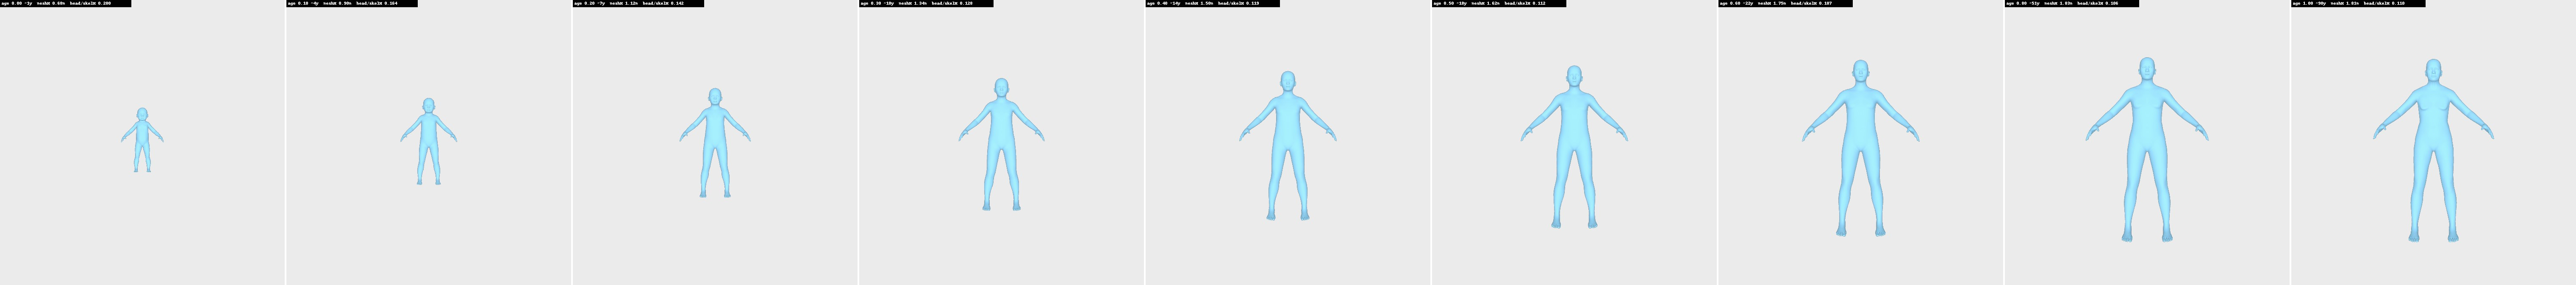
\includegraphics[width=\textwidth]{figures/img/F21_age_sweep.jpg}%
  }{%
    \fbox{\parbox[c][4cm][c]{0.9\textwidth}{\centering
      \TODO{F21 placeholder for \texttt{figures/img/F21\_age\_sweep.jpg}, a copy of
      \texttt{results/diagnostics/bodymodel*/vis/age\_sweep.jpg} from \texttt{diag\_bodymodel.sh}}}}%
  }
  \caption[Anny with age swept from 0 to 1]{Anny at the mean AnnyOne shape in
    rest pose, with only the age value changed from 0 to 1. The skeletal height
    (head joint to mean ankle) grows from \BgSweepHeightAgeZero\,m to
    \BgSweepHeightAgeOne\,m. Body model only, no network; one camera for all
    panels, so the relative size is visible. The approximate years printed in the
    panel titles come from one of three age scales that disagree
    (Section~\ref{sec:bg-bodymodels}) and are not used in this thesis.}
  \label{fig:bg-age-sweep}
\end{figure}

Anny's package also ships a calibration from age values to years. I never convert
ages to years, because three scales are in use and disagree: the value read as
11~years is \BgElevenYearsScaleC{} in Anny's calibration, \BgElevenYearsScaleA{}
in the conversion my code inherited, and \BgElevenYearsScaleB{} on the MakeHuman
slider. I call a person \emph{child-shaped} if the age value is below about
\BgChildShapeAge{}, which selects child-like bodies on any of the three scales.

Two properties of the rig matter later. Of the \BgAnnyBones{} bones,
\BgAnnyHelperBones{} are helper bones (toes, breasts, face micro-bones and similar)
whose rotation an image cannot reveal. I keep them at rest in training, which
leaves \BgAnnyActiveBones{} predicted bones. The neck is modelled by three stacked
bones, \texttt{neck01}, \texttt{neck02} and \texttt{neck03}, followed by
\texttt{head}.

\paragraph{AnnyOne.}
AnnyOne is NAVER's synthetic dataset for Anny: rendered scenes of several people
with exact Anny labels for every person (all bone transforms, all
\BgAnnyPhenotypes{} phenotypes and the camera). Its authors describe more than
\num{\BgAnnyOnePublished} images~\cite{bravo2026annyfit}; the release copy I train on
holds \num{\BgAnnyOneImages} images of \BgAnnyOneRes${\times}$\BgAnnyOneRes{}
pixels, which I resize to \BgInputRes{} pixels for the network.
Chapter~\ref{ch:data} describes its content, its few children and the 100 images
I hold out. AnnyOne is the reason Anny is usable for mesh recovery at all: it is
the only source of complete Anny labels, including shape, that I have.

% -----------------------------------------------------------------------------
\section{Single-person and multi-person human mesh recovery}
\label{sec:bg-hmr}

\paragraph{HMR.}
Human mesh recovery (HMR) regresses body-model parameters from an image.
HMR~\cite{kanazawa2018hmr} did this for one cropped person with a convolutional
encoder and an iterative regressor that refines its own estimate, and it used an
adversarial prior to keep poses plausible when only 2D keypoints supervise them.
My model follows the same principle: a network outputs the parameters directly,
with no optimisation at test time.

\paragraph{SMPLify and SPIN.}
SMPLify~\cite{bogo2016smplify} goes the other way. It fits SMPL to detected 2D
keypoints by optimisation, with pose and shape priors. SPIN~\cite{kolotouros2019spin}
puts such a fit inside the training loop: the network's guess starts the fit, and
the fitted result becomes a better training target. My 3DPW converter
(Chapter~\ref{ch:data}) is an optimisation of the SMPLify kind, but in 3D and
between two body models: it fits Anny's joints to the joints of 3DPW's SMPL
ground truth. Unlike SPIN, the fit runs once, offline, and its output is a
fixed label set.

\paragraph{HMR~2.0 and 4DHumans.}
HMR~2.0~\cite{goel2023humans4d} replaced the convolutional encoder by a Vision
Transformer (ViT)~\cite{dosovitskiy2021vit} with a transformer decoder and showed
that a large ViT trained on a broad data mixture is a strong and simple recipe.
The same work tracks people through video (4DHumans, building on
PHALP~\cite{rajasegaran2022phalp}). Its single-image recipe supports the choice of
a large ViT backbone, which Multi-HMR shares.

\paragraph{ROMP.}
Multi-person methods must also find the people. Two-stage methods run a detector
and then a single-person network on each crop; the cost grows with the number of
people, and each crop loses the context of the others. ROMP~\cite{sun2021romp}
does both in one pass: it predicts a heatmap of body centres and, at every
location, a map of SMPL parameters, and reads the parameters at the detected
centres. Multi-HMR keeps this single-shot idea: one forward pass per image
whatever the number of people.

\paragraph{BEV and Relative Human.}
BEV~\cite{sun2022bev} extends ROMP with an explicit reasoning about depth, so that
people are ordered correctly from near to far, and with an age-aware body: an age
offset blends the adult SMPL template towards an infant one. To train and test
this, the authors collected Relative Human, real photos in which every person
carries an age group (adult, teenager, kid, baby), a depth layer and keypoints.
BEV relates to two choices of mine. Its depth focus mirrors the depth defect I
found (Chapter~\ref{ch:diagnostics}): a mesh error measured after centring the
pelvis cannot see where a person is placed. And Relative Human is the only real
data with age labels I could use, so I use it, for evaluation only, to test
whether predicted ages and genders follow the people on real photos
(Chapter~\ref{ch:results}). Relative Human has no 3D bodies, so it can test age
groups and gender but not shape values.

\paragraph{Multi-HMR.}
Multi-HMR~\cite{baradel2024multihmr} is the architecture of this thesis. A ViT
backbone initialised from DINOv2~\cite{oquab2023dinov2} turns the image into one
token per $\BgPatch{\times}\BgPatch$-pixel patch; at \BgInputRes{} pixels this is a
$\BgTokenGrid{\times}\BgTokenGrid$ grid. For each token a small head predicts
a score that a person's primary keypoint lies in this patch, and a 2D offset
inside the patch. In the released code the primary keypoint is the head
joint~\cite{naver2024multihmrcode}. Tokens with a high score become the queries of
the \emph{Human Perception Head} (HPH): a few blocks in which the queries attend
to each other and, by cross-attention, to all image tokens. The image tokens are
joined with a Fourier encoding of each patch's viewing ray, computed from the
camera intrinsics, so the head knows the camera. For every query the HPH regresses
the body-model parameters and the person's distance from the camera; the 3D
position follows by back-projecting the detected head pixel to that distance. I
kept this design and changed what comes out of it (Chapter~\ref{ch:method}).
The distance belongs to the head joint, and this anchor is at the centre of the
depth defect of Chapter~\ref{ch:diagnostics}.

The authors trained Multi-HMR on synthetic data, mainly BEDLAM~\cite{black2023bedlam}
and AGORA~\cite{patel2021agora}, together with their own close-up set CUFFS. The
project page lists the released SMPL-X checkpoints with their per-vertex error
(PVE) on the 3DPW test set and their run time on a V100
GPU~\cite{naver2024multihmrcode}. At \BgInputRes{} pixels, the ViT-L checkpoint
reaches \BgMhrLPVE\,mm in \BgMhrLMs\,ms, the ViT-B checkpoint \BgMhrBPVE\,mm in
\BgMhrBMs\,ms and the ViT-S checkpoint \BgMhrSPVE\,mm in \BgMhrSMs\,ms; a ViT-L at
896 pixels reaches \BgMhrLEightNineSixPVE\,mm in \BgMhrLEightNineSixMs\,ms. On
BEDLAM validation the gap between ViT-L and ViT-B is larger,
\BgMhrLBedlamPVE{} against \BgMhrBBedlamPVE\,mm. Two things follow for this
thesis. A ViT-B backbone loses little on real 3DPW images and runs in \BgMhrBMs{}
instead of \BgMhrLMs\,ms, which is why my smaller model is a ViT-B student and not a ViT-S one
(Section~\ref{sec:bg-kd}). And these numbers are SMPL-X errors against 3DPW's own
SMPL ground truth; they cannot be compared with the Anny-space errors of this
thesis.

\paragraph{Multi-HMR-Anny, NAVER's Anny checkpoint.}
In February 2026 NAVER released a Multi-HMR checkpoint that predicts Anny
(\texttt{multiHMR\_672\_L\_anny}): a ViT-L backbone at \BgInputRes{} pixels, trained
on BEDLAM, AnnyOne and further real images~\cite{naver2024multihmrcode}. A
multi-person HMR network that predicts Anny therefore already exists, and this
thesis does not claim to be the first. This checkpoint, called Multi-HMR-Anny in this
thesis, matters in three ways. It is where my model comes from: the backbone
weights of my whole model line were taken from it (Chapter~\ref{ch:method}). It
is the baseline I compare against, evaluated with my code on my labels
(Chapter~\ref{ch:results}, Section~\ref{sec:res-baseline}). And it differs from my
model in its head: its decoder has \BgNaverHeadLayers{} cross-attention blocks and
\BgNaverHeadParams\,M parameters, against \BgOurHeadLayers{} blocks and
\BgOurHeadParams\,M in mine, on the same backbone. In its released inference code
the predicted 3D position is applied at the head joint, the same joint the
detection refers to. The checkpoint has its own licence file, separate from
Anny's. NAVER trained it on AnnyOne, which includes the images I hold out, so its
AnnyOne error is most likely an in-sample number; Chapter~\ref{ch:results} states
this next to every comparison.

\paragraph{Anny-Fit.}
Anny-Fit~\cite{bravo2026annyfit}, by the same group, refines Multi-HMR's Anny
predictions per image by optimisation, guided by off-the-shelf semantic, depth,
keypoint and segmentation cues, and adapts adult-only models to children without
retraining. It targets the weakness I measure on real photos, children with adult
bodies, but at test time, while my model stays a single forward pass. I did not
use it; it is the natural comparison for future work on children.

% -----------------------------------------------------------------------------
\section{Synthetic training data}
\label{sec:bg-synthetic}

AGORA~\cite{patel2021agora} renders scanned people with SMPL-X fits into
realistic scenes, children included. BEDLAM~\cite{black2023bedlam} renders
animated SMPL-X bodies with simulated clothing and showed that synthetic images
alone can train competitive networks. AnnyOne does the same for Anny. Synthetic
labels are exact and complete, shape included, but leave open how well a network
transfers to real photos. In this thesis the question is concrete: on the
synthetic holdout my shape predictions follow the labels, on real photos they
collapse towards the training average (Chapter~\ref{ch:diagnostics}). This is why
the final model mixes real images into every batch (\BgMixReal\,\%), and why
those images need Anny labels.

% -----------------------------------------------------------------------------
\section{Real-data labels for a new body model}
\label{sec:bg-labels}

\paragraph{Why 3DPW needs a conversion.}
3DPW~\cite{vonmarcard2018_3dpw} is the standard real-world test set for mesh
recovery. It holds \BgThreeDPWSequences{} outdoor video sequences filmed with a
moving phone camera; body-worn inertial sensors and the video together give SMPL
ground truth for the one or two actors of each sequence. People walking by are
not labelled. The ground truth exists only in SMPL. SMPL and Anny share neither
their skeleton nor their shape space: the joint positions differ, the bone
hierarchy differs, and SMPL's statistical coefficients have no mapping onto
Anny's named phenotypes. To train or test an Anny network on 3DPW, the labels
must therefore be re-expressed in Anny, by fitting.

\paragraph{Existing tools.}
The SMPL-X code includes a tool that transfers fits between SMPL-family models
through a fixed vertex correspondence~\cite{pavlakos2019smplx}, and the Anny
package offers SMPL-X-compatible topologies and an inverter that fits Anny to a
target mesh~\cite{naver2025annycode}. None turns a 3DPW label into an Anny label
directly, and I did not evaluate the inverter. I wrote my own converter: it fits
Anny's joints to the 3D joints of the 3DPW ground truth frame by frame, then fixes
one body per person and fits the pose again (Chapter~\ref{ch:data}, with the
three defects I later found and the independent check of the corrected labels).

\paragraph{What converted labels can and cannot supervise.}
A fit to joint positions recovers what joint positions determine and nothing
more. The converted labels supervise the root position and rotation, the bones
between the mapped joints, gender (from 3DPW's metadata) and one height and one
proportions value per person. They cannot supervise muscle, weight, cup size,
firmness or the three ethnicity blends, which joint positions do not reveal.
Age is not fitted either; 3DPW shows only adults. In my labels age is the
constant \BgFixedAge{} and the \BgFixedPhenotypes{} others are 0.5, so
\BgConstPhenotypes{} of the \BgAnnyPhenotypes{} phenotypes are constants. Of the
\BgAnnyBones{} bones, \BgRestBones{} stay at rest by design, including
\texttt{neck02}, \texttt{neck03}, \texttt{head} and every finger bone: SMPL's
\BgSmplJoints{} joints constrain only the bones mapped onto them, and 3DPW's SMPL
ground truth has no finger joints. The fit
itself leaves an error floor of about \BgFitFloor\,mm on the body joints. Three
consequences run through the thesis. On 3DPW only pose, gender, height and
proportions are tested, not full shape. Training on the converted labels pulls
the eight constant phenotypes towards their constants on real images, which
Chapter~\ref{ch:results} measures. And errors on these labels are Anny-space
errors over Anny joints with a conversion floor, not comparable with published
3DPW results.

\paragraph{Attribute labels as an alternative.}
SHAPY~\cite{choutas2022shapy} supervises body shape on real images with
measurements and crowd-sourced word attributes instead of 3D ground truth.
Anny's named phenotypes would suit such labels; I collected none and rely on the
age groups and genders of Relative Human, two of the \BgAnnyPhenotypes{} values.

% -----------------------------------------------------------------------------
\section{Knowledge distillation}
\label{sec:bg-kd}

\paragraph{Output distillation.}
Knowledge distillation~\cite{hinton2015distilling} trains a small \emph{student}
network to reproduce a large, trained \emph{teacher}. In the original form the
student matches the teacher's class probabilities, both softened by a
temperature $T$, with a Kullback--Leibler (KL) divergence:
\begin{equation}
  \mathcal{L}_{\mathrm{KD}} \;=\; T^2\, \mathrm{KL}\!\left(\mathrm{softmax}(\mathbf{z}_t/T)\,\big\|\,\mathrm{softmax}(\mathbf{z}_s/T)\right),
  \label{eq:bg-kd}
\end{equation}
where $\mathbf{z}_t$ and $\mathbf{z}_s$ are the teacher's and the student's
outputs before the softmax. A higher $T$ spreads the probabilities and exposes
how the teacher ranks the wrong answers; the factor $T^2$ keeps the gradient size
independent of $T$. Mesh recovery regresses numbers rather than classes, so the
output part of my distillation is a plain L1 distance between the student's and
the teacher's bone rotations, phenotypes and depth.

\paragraph{Feature distillation.}
FitNets~\cite{romero2015fitnets} let the student also match an intermediate
representation of the teacher, through a small learned regressor that bridges the
different widths. My student does the same at the end of the backbone: a linear
projector maps its \BgProjIn-wide ViT-B tokens to the teacher's \BgProjOut-wide
tokens, and a KL term at $T=\BgKDTemperature$, in the form of
Equation~\eqref{eq:bg-kd} applied to the projected tokens, pulls them towards the
teacher's. Because the projected tokens have the teacher's width, the teacher's
trained detection and HPH heads can be copied into the student unchanged and
fine-tuned, instead of being trained from scratch. Chapter~\ref{ch:method} gives
the recipe.

\paragraph{DINOv2.}
DINOv2~\cite{oquab2023dinov2} trained its largest ViT with self-supervision and
distilled the smaller ViTs from it, so a DINOv2 ViT-B is a good starting point for
a student. The question for this thesis is whether a ViT-B student of my final
ViT-L model keeps at least \BgNinetyFive\,\% of its accuracy on both test sets,
the bar my supervisor set for a smaller model. The student has
\BgStudentParams\,M parameters against \BgFinalParams\,M, a factor of
\BgStudentParamRatio{} fewer.

% -----------------------------------------------------------------------------
\section{Temporal models for video}
\label{sec:bg-temporal}

My model works on single frames. The temporal requirement of the thesis asks
whether motion in video can be used. This work has not started, so this section
only names the methods a frame-wise model like mine could build on. Most refine
per-frame features of a frozen image network, the form that would sit on top of
my per-person HPH tokens.

\paragraph{HMMR.}
HMMR~\cite{kanazawa2019hmmr} runs a temporal convolution over per-frame features
and predicts the current, past and future poses. It showed that a short window
already smooths the motion.

\paragraph{VIBE.}
VIBE~\cite{kocabas2020vibe} adds a recurrent network over per-frame features and
a motion discriminator trained on motion capture. The discriminator is tied to
SMPL; for Anny it would need Anny motion data.

\paragraph{TCMR.}
TCMR~\cite{choi2021tcmr} found that a strong per-frame feature lets the temporal
model ignore its neighbours, which causes jitter. It adds branches that predict
the current frame from past and future frames alone and lowers the acceleration
error, the jitter measure I would use as well.

\paragraph{MPS-Net and GLoT.}
MPS-Net~\cite{wei2022mpsnet} replaces the recurrence by attention over frames.
GLoT~\cite{shen2023glot} combines a global transformer over a long window,
trained by masking poses, with a local one over neighbouring frames. Both refine
per-frame features, as a refiner on my model would.

\paragraph{SmoothNet.}
SmoothNet~\cite{zeng2022smoothnet} removes jitter from the output poses of any
estimator without image features. It needs no change to my model, so it is the
baseline a learned refiner would have to beat.

\paragraph{PHALP, 4DHumans and WHAM.}
PHALP~\cite{rajasegaran2022phalp} tracks people by predicting their 3D
appearance, location and pose into the next frame; 4DHumans~\cite{goel2023humans4d}
combines it with HMR~2.0. Tracking is the step any multi-person video method needs
first. WHAM~\cite{shin2024wham} places the motion in world coordinates using the
camera's rotation and foot contact, which addresses a problem my model shares:
per-frame depth that is not consistent over time.

% -----------------------------------------------------------------------------
\section{What this thesis adds}
\label{sec:bg-gap}

NAVER's Multi-HMR-Anny already predicts Anny for several people in one image.
What was missing is knowledge of how such a model fails on real images, why, and
how far it can be repaired, together with real labels to measure it in Anny space
and a smaller model of comparable accuracy. This thesis contributes the
following. Each item is stated against that baseline and names the chapter with
the evidence.

\paragraph{A measured diagnosis of three failures.}
The model I started from showed thin, twisted necks, claw-like fingers and
children with adult bodies. Before changing anything I tested what is not the
cause (labels, rig, gradients, optimiser), and then traced each failure to a
specific mechanism (Chapter~\ref{ch:diagnostics}).

\paragraph{The depth-anchor fix.}
The network places each person by the head, but my training targets were built at
the pelvis. The 2D losses reconciled the two by pushing bodies away and drawing
them too small, which the pelvis-centred mesh error could not see. Building the
targets at the anchor joint nearly halves the error of the body's 3D position against a
matched control (Chapters~\ref{ch:method} and~\ref{ch:results}).

\paragraph{The bone correction.}
Two neck bones and two hand bones were turned by half a turn in every checkpoint
of my model line. A constant rotation applied at the output, estimated once and
with no parameters, turns them back and restores the neck's thickness; its origin
is unknown (Chapters~\ref{ch:diagnostics} and~\ref{ch:method}).

\paragraph{Converted 3DPW labels with a verified check.}
I converted 3DPW's SMPL ground truth to Anny for all \BgThreeDPWPeople{} actors,
found three defects in the first label set (reversed gender, a missing actor in
two-person frames, missing images), fitted all actors again and checked the new
labels with an independent test (Chapter~\ref{ch:data}). This is what makes
training on real images and Anny-space evaluation on 3DPW possible.

\paragraph{The final model and its control.}
The final model, called Final from Chapter~\ref{ch:method} on, combines both fixes with \BgMixReal\,\% real images in every batch.
A control run with the same data, steps and start but without the two fixes
separates what the fixes do from what the extra training does
(Chapter~\ref{ch:results}).

\paragraph{The baseline comparison.}
I evaluated Multi-HMR-Anny with my own code, settings and labels, so that both
models are measured the same way on AnnyOne and on 3DPW
(Section~\ref{sec:res-baseline}).

\paragraph{The smaller student.}
A ViT-B student (Student) distilled from the final model, with \BgStudentParamRatio{} times
fewer parameters, is the route to the requirement of a model that is not exactly
Multi-HMR (Section~\ref{sec:res-student}).
